

\chapter{Cryptography}
%Quick overview of cryptography

\section{Algorithm selection overview}
%Which encrypting plan will I use?

\subsection{Symmetric key encryption}
\paragraph{Selecting an algorithm, among so many, was pretty straightforward given my use case, but I wanted to show my thought processes. Firstly, there are two fundamental paths for selecting an encryption algorithm. The selection between \emph{asymmetric} and \emph{symmetric} key encryption is the initial decision.}

\begin{enumerate}
\item Asymmetric-key cryptography: A public and private key are created by both people wanting to exchange encrypted emails. This is the most secure and most commonly implementated encryption available, popularly known as "public-key encryption." Examples encryption key algorithms used include RSA and Diffe-Hellman-Merkle.
There are challenges though:\cite{book0}
\begin{enumerate}
\item Both parties need to create their own keys
\item Keys need to be exchanged, i.e. a person has to be acute enough to search for the other person's public key -- assuming one even exists
\item Additional client software is also often required
\end{enumerate}
\item Symmetric-key Encryption: use the same key for both encryption and decryption\cite[p. 155]{book1}
\begin{enumerate}
\item The primary drawback is that both parties will need to exchange that key, often times in the form of a password.
\end{enumerate}
\end{enumerate}

\paragraph{The goal of this project is \emph{ease of use} (at the cost of security), so our choice is clear: symmetric-key encryption.}

\subsection{Block vs. Stream cipher encryption}
\paragraph{Next, we need to decide between a block cipher or a stream cipher. As Bruce Schneier defines the two in his book "Applied Cryptography: Protocols, Algorithms in C" as:}

\begin{quote}
There are two basic types of symmetric algorithms: block ciphers and stream ciphers. Block ciphers
operate on blocks of plaintext and ciphertext—usually of 64 bits but sometimes longer. Stream
ciphers operate on streams of plaintext and ciphertext one bit or byte (sometimes even one 32-bit
word) at a time. With a block cipher, the same plaintext block will always encrypt to the same
ciphertext block, using the same key. With a stream cipher, the same plaintext bit or byte will
encrypt to a different bit or byte every time it is encrypted.\cite[p. 12]{book2}
\end{quote}
\paragraph{The advantages of a stream ciphers:}\footnote{https://crashtest-security.com/block-cipher-vs-stream-cipher/}

%TODO resume here, giving highlight to stream without reason. Instead, mention that by now, mixed algorithms are also possible -if not, prevalent.

\begin{itemize}
\item bit or byte at a time encryption
\item speed of encryption/decryption
\end{itemize}

\paragraph{are more appropriate for hardware implementations.}

\paragraph{According to Bruce Schneier, block ciphers are more suitable for software implementation as they are easier to implement, avoid time-consuming bit manipulations, and operate on computer sized blocks.}\cite[p. 172]{book2}

\subsection{Block cipher selection}
\paragraph{There are many block ciphers to choose from, these are just some of the most popular:}\cite{book3}
\begin{enumerate}
\item Digital Encryption Standard(DES): DES is a symmetric key block cipher that uses 64-bit blocks, but it has been found vulnerable to powerful attacks. This is the reason the use of DES is on a decline. 
\item Triple DES:This symmetric key cipher uses three keys to perform encryption-decryption-encryption. It is more secure than the original DES cipher but as compared to other modern algorithms, triple DES is quite slow and inefficient. 
\item Advanced Encryption Standard(AES): AES has superseded the DES algorithm and has been adopted by the U.S. government. It is a symmetric key cipher and uses blocks in multiple 32 bits with minimum length fixed at 128 bits and maximum at 256 bits. The algorithm used for AES, was originally named Rijndael.\footnote{The winners of the AES competition were two Belgians: Vincent Rijmen, Joan Daemen, thus the algorithm's name: "\textbf{Ri}n\textbf{jdae}l"}
\item Blowfish: Blowfish is a symmetric key block cipher with a block size of 64 and a key length varying from 32 bits to 448 bits. It is unpatented, and the algorithm is available in the public domain. 
\item Twofish: Twofish is also a symmetric key block cipher with a block size of 128 bits and key sizes up to 256 bits. It is slower than AES for 128 bits but faster for 256 bits. It is also unpatented and the algorithm is freely available in the public domain.
\end{enumerate}

\paragraph{But, after an overall account of the block enciphers available, the author decided there is really only one reasonable choice: the Advanced Encryption Standard (AES). This decision is based }

\section{Advanced Encryption Standard (AES)}

\paragraph{AES is basically the only choice for a block cipher scheme. It has been the industry standard for the past 20 years, even used by the U.S. government.}\cite{book4}

%TODO what is my reasoning for selecting AES?
%AES is derived from a competition from 1997, spanning world wide competitors. A belgian team won, an
% Which mode of choose, why??
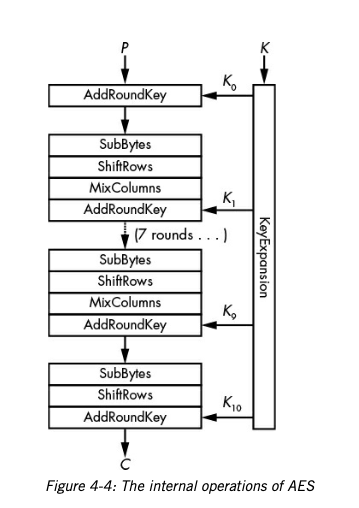
\includegraphics[width=0.9\textwidth]{AES-image.png}